\chapter{Methodology and Contributions}

\section{Introduction}
\label{sec:contribution-introduction}

In this chapter, we present the core contributions of our work on automated brain tumor detection in magnetic resonance (MR) images. Building upon the BraTS benchmark dataset \cite{Menze2015}, our pipeline integrates a deep learning–based segmentation module with a classical machine learning classifier and culminates in a user‐friendly demo application. The main objectives of this chapter are:
\begin{itemize}
  \item To describe a tailored U-Net–based segmentation pipeline for delineating tumor subregions in MRI slices.
  \item To detail a feature‐extraction and SVM classification scheme that distinguishes high‐grade from low‐grade gliomas using volumetric, intensity, texture, and shape descriptors.
  \item To demonstrate the integration of these modules within an end-to-end application for streamlined inference on new patient data.
\end{itemize}

The remainder of this chapter is organized as follows. In Section~\ref{sec:contribution-dataset}, we introduce the dataset and preprocessing steps. Section~\ref{sec:contribution-segmentation} details the U-Net segmentation module, including architecture and training protocol. Section~\ref{sec:contribution-classification} covers the feature engineering and SVM classification. Section~\ref{sec:contribution-demo} presents the design and functionality of our demo application. We conclude with a discussion of key findings and future directions.

\section{Proposed Framework Overview}
\label{sec:contribution-framework}
In this section, we look at our proposed fremework from a systematic perspective. The framework is designed to perform end-to-end brain tumor segmentation and classification. We will discuss the design of the final pipeline and the training workflow to achieve the desired results.

\subsection{End-to-End Inference Pipeline}
The purpose of our project is to have an end-to-end inference pipeline accepts a raw MR image as input, applies preprocessing steps, performs segmentation of the tumor region using the trained U-Net model, classifies the tumor grade via the SVM classifier, and finally outputs the original image overlaid with the segmentation mask along with the predicted grade.
\begin{figure}[H]
  \centering
  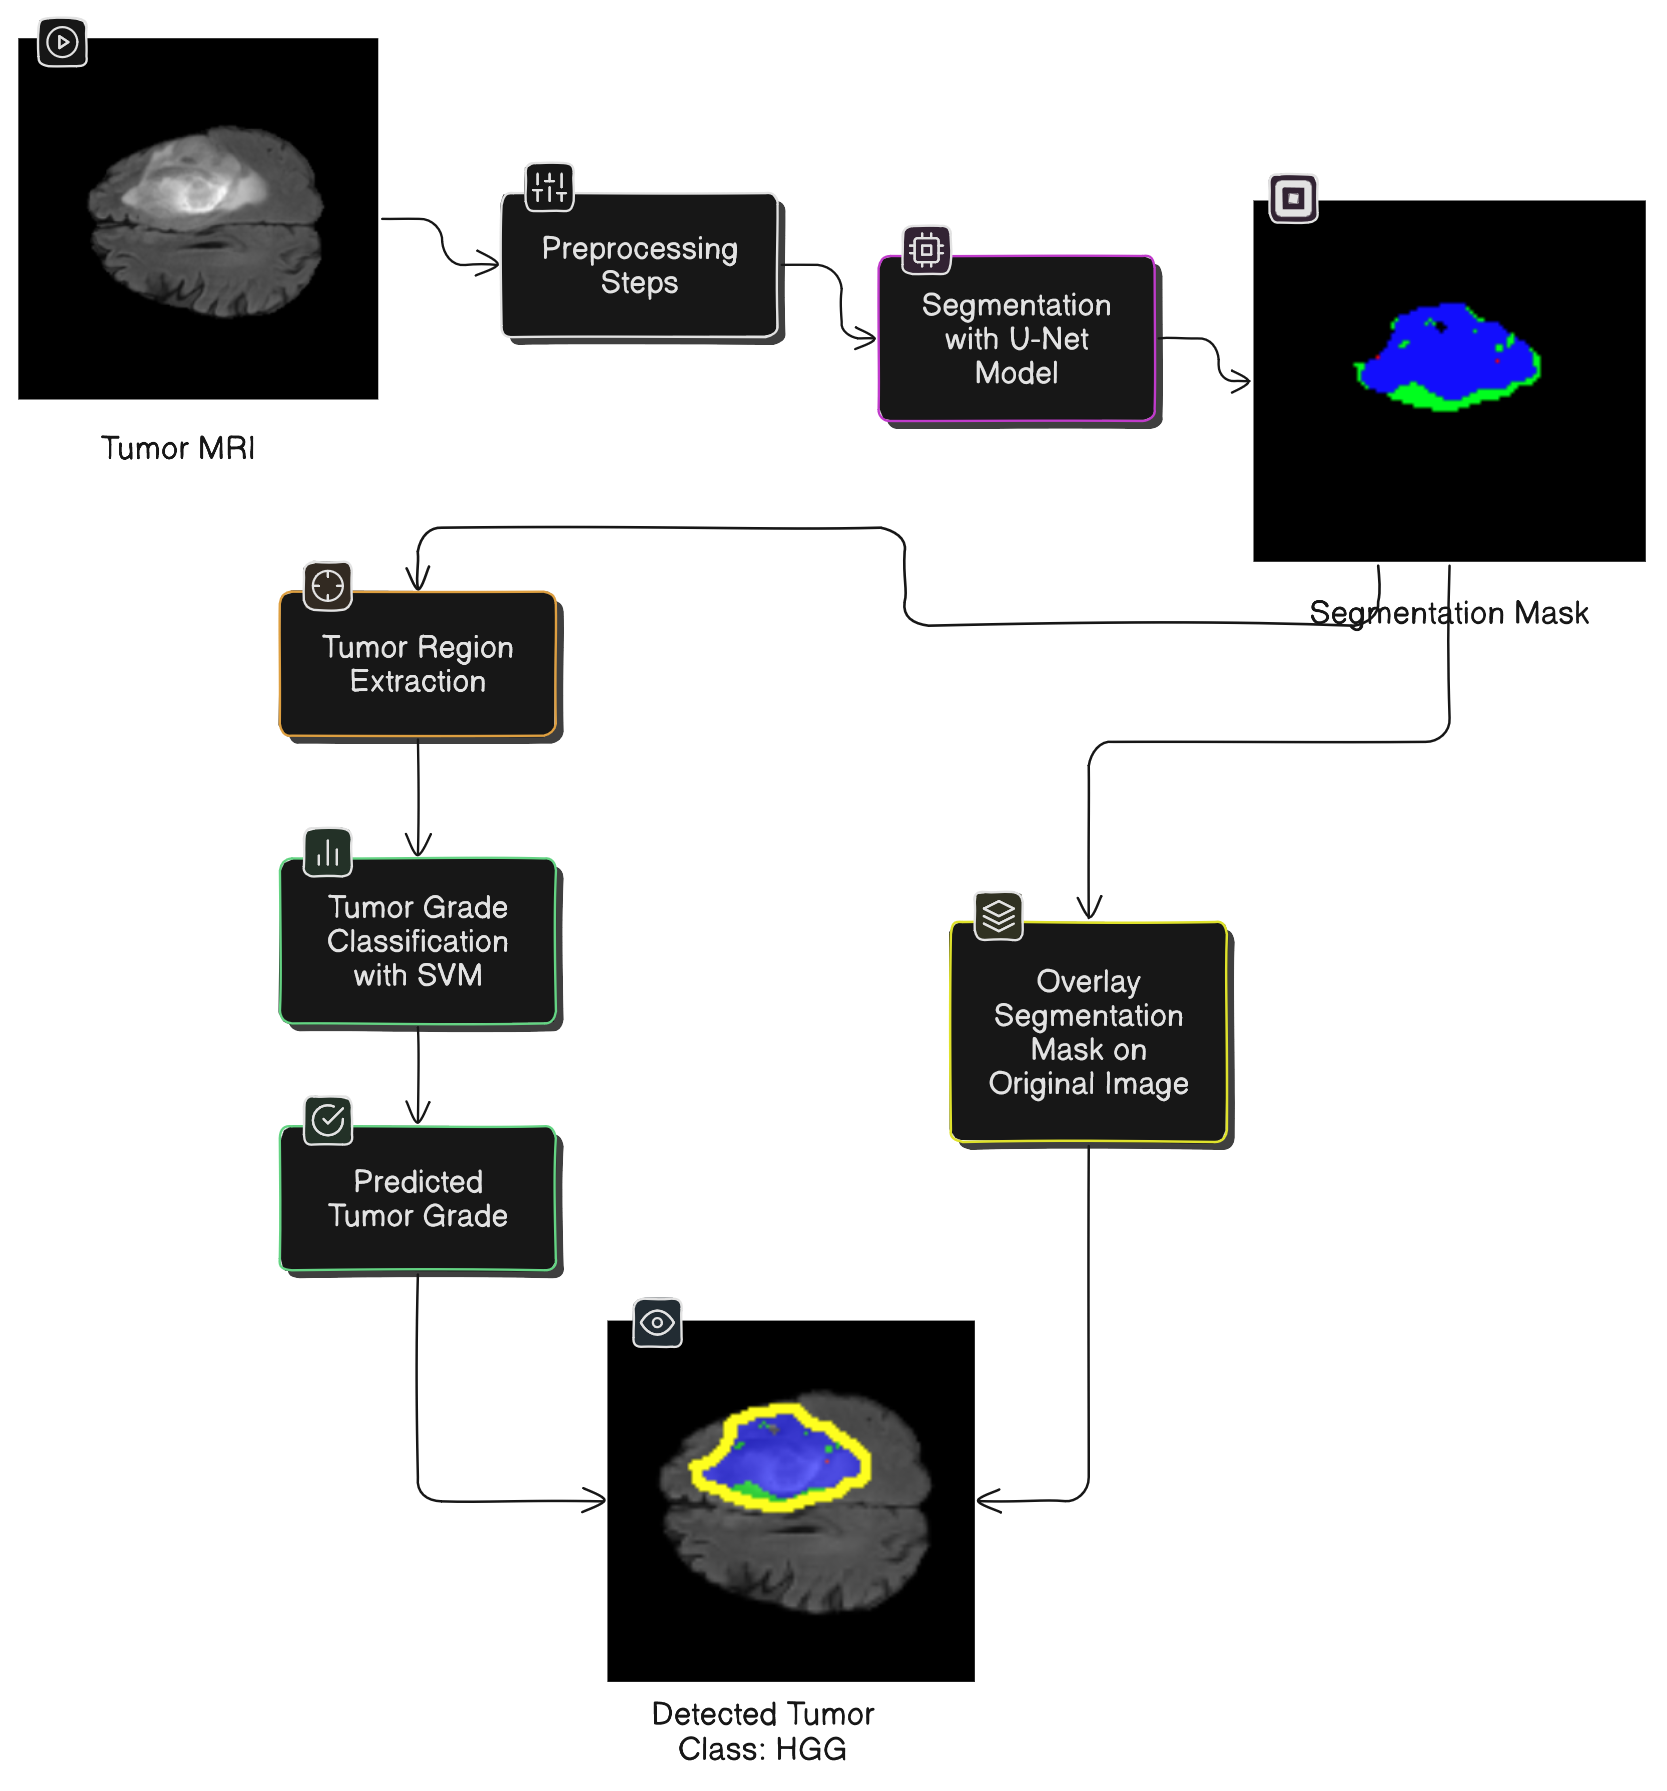
\includegraphics[width=0.8\textwidth]{Images/Chapter3/pipeline.png}
  \caption{Overview of the end-to-end inference pipeline.}
  \label{fig:pipeline}
\end{figure}


\subsection{Model Training Workflow}
The training workflow begins with the BraTS dataset. After preprocessing and augmentation, the data is split into training, validation, and test sets. We then train the U-Net segmentation model in parallel with feature extraction followed by SVM classifier training, yielding two standalone models for inference.

\begin{figure}[H]
  \centering
  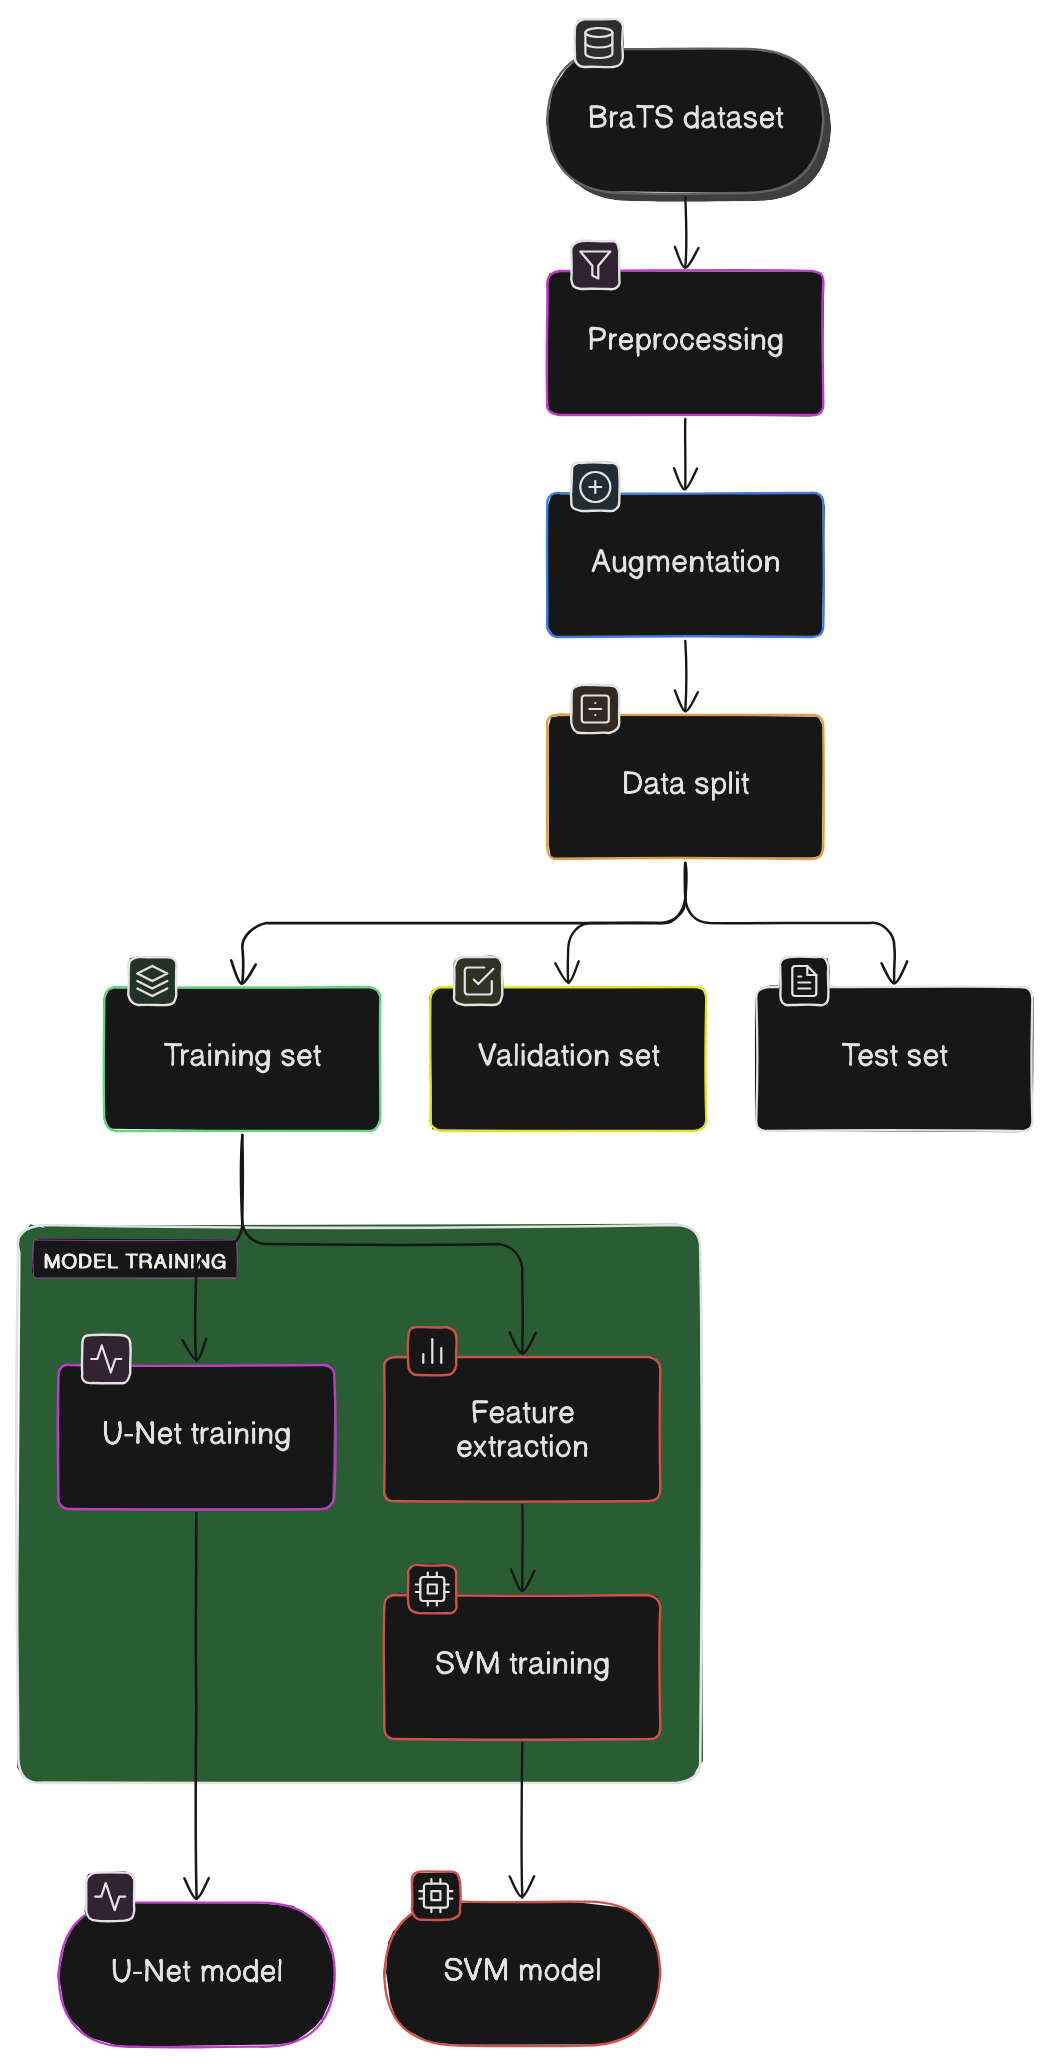
\includegraphics[width=0.6\textwidth]{Images/Chapter3/training.png}
  \caption{Overview of the training workflow.}
  \label{fig:training}
\end{figure}

\section{Dataset and Preprocessing}
\label{sec:contribution-dataset}
In order to train our hybrid model we used the Brain Tumor Segmentation (BraTS) 2020 dataset, which is a collection of multimodal Magnetic Resonance Imaging (MRI) scans used for the segmentation of brain tumors.

\subsection{BraTS Dataset Description}
The dataset includes MRI scans from glioma patients, providing four different MRI modalities per patient:
\begin{enumerate}
  \item \textbf{Native (T1)}
  \item \textbf{Post-contrast T1-weighted (T1ce - contrast enhanced)}
  \item \textbf{T2-weighted (T2)}
  \item \textbf{T2-FLAIR (T2 - Fluid Attenuated Inversion Recovery)}
  \item \textbf{Tumor Segmentation Mask}
\end{enumerate}
\begin{figure}[H]
  \centering
  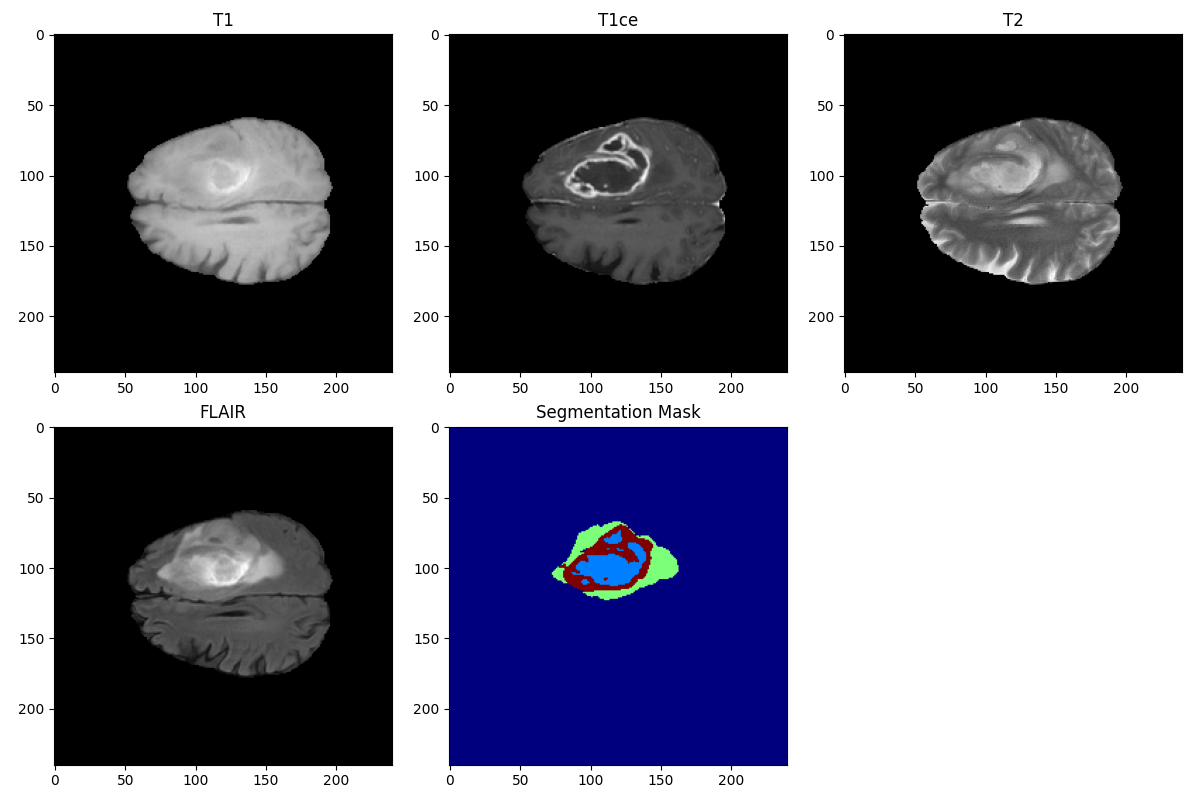
\includegraphics[width=0.8\textwidth]{Images/Chapter3/modalities.png}
  \caption{Brats modalities: T1, T1ce, T2, and T2-FLAIR.}
  \label{fig:modalities}
\end{figure}

These scans come with expert-annotated segmentation masks that delineate the tumor into various sub-regions, such as the necrotic and non-enhancing tumor core, the peritumoral edema, and the enhancing tumor. Research has demonstrated that accurate segmentation is linked to improved prognostic assessments and treatment outcomes.

\begin{itemize}
  \item \textbf{Class 0 (Not Tumor):} This class represents normal brain tissue or background, where no tumor tissue is present.
  \item \textbf{Class 1 (Non-Enhancing Tumor):} This class corresponds to the necrotic or non-enhancing core regions of the tumor. These areas typically lack contrast enhancement and may include dead or less active tumor tissue.
  \item \textbf{Class 2 (Edema):} This class identifies regions of peritumoral edema, which is the swelling around the tumor caused by fluid accumulation. Edema is important for understanding the extent of the tumor’s impact on surrounding brain tissue.
  \item \textbf{Class 4 (Enhancing Tumor):} This class captures the actively enhancing parts of the tumor, visible after the administration of a contrast agent. These regions often indicate aggressive tumor tissue with increased blood flow and permeability.
\end{itemize}

To visually interpret these segmentations, we map the categorical labels to a custom colormap. In our example, we use four distinct colors to represent:

\begin{figure}[H]
  \centering
  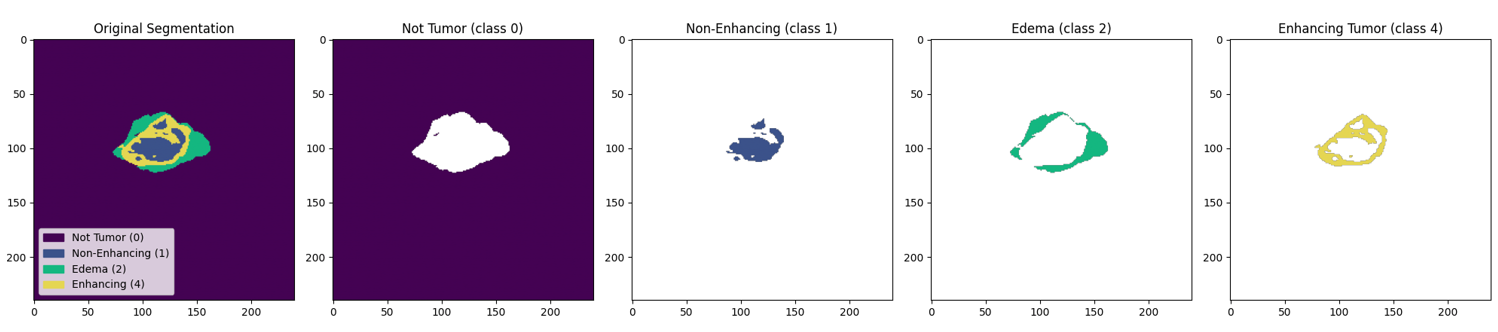
\includegraphics[width=1.1\textwidth]{Images/Chapter3/tclass.png}
  \caption{Segmentation of Tumor classes.}
  \label{fig:tclass}
\end{figure}

\subsection{Preprocessing}
\begin{enumerate}
  \item \textbf{Slice Selection:} Extract 100 axial slices per volume, starting at slice index 22 to avoid low‐information regions.
  \item \textbf{Resizing:}
        \begin{itemize}
          \item MRI slices $\to$ \texttt{128$\times$128} for U-Net input.
          \item Segmentation masks $\to$ \texttt{240$\times$240} before one‐hot encoding.
        \end{itemize}
  \item \textbf{Normalization:} Intensity values scaled by the global maximum per volume.
  \item \textbf{Augmentation:} Random flips (horizontal, vertical) and rotations (0°, 90°, 180°, 270°) applied on-the-fly during training.
\end{enumerate}

% No new BibTeX entries beyond those in the Introduction.
